% DOCUMENT CLASS
\documentclass[11pt]{article}
%PACKAGES
\usepackage[utf8]{inputenc}
\usepackage[ngerman]{babel}
\usepackage[reqno,fleqn]{amsmath}
\setlength\mathindent{10mm}
\usepackage{amstext}
\usepackage{amssymb}
\usepackage{fancyhdr}
% Grafik
\usepackage{graphicx}
\usepackage{subfigure}
\usepackage{wrapfig}
% Zahlenwerte mit Einheiten mittels \unit{Zahlenwert}{Einheit}
\usepackage[thinspace,thinqspace,squaren,textstyle]{SIunits}
% FORMATIERUNG
\usepackage[paper=a4paper,left=25mm,right=25mm,top=25mm,bottom=25mm]{geometry}
\setlength{\parindent}{0cm}
\setlength{\parskip}{1.5mm plus1mm minus1.5mm}
% PAGESTYLE
\pagestyle{fancy}
\setlength\headheight{30pt}
\lhead{Michael Hufschmidt, Mat. Nr. 6436122\\Florian Jochheim, Mat. Nr. 6508131}
\rhead{Übungen zur Physik IV, SoSe 2015\\Blatt 04 zum 04.05.2015}
%MATH SHORTCUTS
\newcommand*{\NN}{\mathbb N}

\begin{document}
\subsection*{Aufgabe 8}
\subsubsection*{a)}
Gegeben seien zwei einzelne Ne-Atome im Abstand $r$. Duch die induzierten
Dipolmomente "`sieht"' jedes Atoms das andere als Lennard-Jones-Potential der Form
\begin{align}
  \varphi(r)_{LJ} = 4 \varepsilon \left[ \left(\frac{\sigma}{r}\right)^{12} -
    \left(\frac{\sigma}{r}\right)^{6} \right]
\end{align}
Die Parameter $\varepsilon$ und $\sigma$ hängen nur von der Atomsorte ab.
In einem Kristall mit $N$ Atomen mit dem Abstand $r_{ij}$ zwischen dem
$i$-ten und $j$-ten Atom muss das Lennard-Jones-Potential über alle Atome
aufsummiert werden. Damit wird die gesamte potentielle Energie $U$:
\begin{align}
\label{eq-U}
  U = \frac{1}{2} N \sum_{i \ne j} 4 \varepsilon
  \left[ \left(\frac{\sigma}{r_{ij}}\right)^{12} -
  \left(\frac{\sigma}{r_{ij}}\right)^{6} \right]
\end{align}
Der Faktor 1/2 stellt sicher, dass jedes Atom nur einmal gezählt wird.
Gleichung \eqref{eq-U} lässt sich vereinfachen mit der Einführung von
(dimensionslosen) Gittersummen
\begin{align*}
  A_6 & = \left . \sum_{i \ne j} \left(\frac{R}{r_{ij}}\right)^6 \right .\qquad
  A_{12} = \sum_{i \ne j} \left(\frac{R}{r_{ij}}\right)^{12}
\end{align*}
die nur noch von der Struktur des Gitters abhängen.  Dabei ist $R$ derAbstand
zum nächsten Nachbarn. Das ergibt für die potentielle Energie:
\begin{align}
\label{eq-U2}
  U(R) = \frac{1}{2} N \varepsilon \cdot \left[ A_{12} \left(\frac{\sigma}{R}\right)^{12} -
  A_6 \left(\frac{\sigma}{R}\right)^{6} \right] =
  \frac{1}{2} N \varepsilon \cdot \left( A_{12} \sigma^{12} R^{-12} -
  A_6 \sigma^6 R^{-6} \right)
\end{align}
Im Gleichgewichtsabstand $R_0$ hat $U(R)$ ein Minimum, dazu differenzieren
wir \eqref{eq-U2}:
\begin{align}
\label{eq-DU}
  \frac{\mathrm{d}}{\mathrm{d} R} U(R) = - \frac{1}{2} N \varepsilon \cdot
    \left(12 A_{12} \sigma^{12} R^{-13} - 6 A_6 \sigma^6 R^{-7} \right)
\end{align}
Nullsetzen von \eqref{eq-DU} liefert schließlich:
\begin{align}
  \nonumber
  \left. \frac{\mathrm{d}}{\mathrm{d} R} U(R) \right|_{R_0} = 0 \quad& \Rightarrow\;
  12 A_{12} \sigma^{12} R_0^{-13} = 6 A_6 \sigma^6 R_0^{-7} \quad \Rightarrow\;
  2 A_{12} \sigma^6 R_0^{-6} = A_6 \\
  \label{eq-R0}
  \;& \Rightarrow\; R_0 = \left(\frac{2 \cdot A_{12}}{A_6}\right)^{1/6} \cdot \sigma
\end{align}

\subsubsection*{b)}
Die Bindungsenergie $u(R)$ pro Atom im Gleichgewichtsabstand $R_0$
ergibt sich aus \eqref{eq-R0} eingesetzt in \eqref{eq-U2}:
\begin{align*}
  u(R_0) &:= \frac{U(R_0)}{N} = \frac{1}{2} \varepsilon \left[ A_{12}  \left(
  \left(\frac{2 \cdot A_{12}}{A_6}\right)^{1/6}\right)^{-12} -
  A_6 \left(
  \left(\frac{2 \cdot A_{12}}{A_6}\right)^{1/6} \right)^{-6}
  \right] =  - \frac{A_6^2}{2 \cdot A_{12}} \cdot  \varepsilon
\intertext{Mit den Zahlenwerten aus dem Aufgabenblatt wird die Bindungsenergie pro Atom}
  u(R_0) &= - 8,610161 \cdot \varepsilon = -\unit{26,69}{\milli\electronvolt}
 \intertext{und für den Gleichgewichtsabstand $R_0$ eines Atoms zum nächsten Nachbarn
 ergibt Gleichung \eqref{eq-R0}:}
 R_0 &=1,0902 \cdot \sigma = \unit{303,07}{\pico\meter}
\end{align*}

\subsubsection*{c)}
In der harmonischen Näherung für Gitterschwingungen $x := R - R_0$ um den
Gleichgewichtszustand $R_0$ macht man eine Taylor-Entwicklung für das
Lennard-Jones-Potential bis zum zweiten Grad:
\begin{align*}
  u(x) = u(R - R_0) = \left. u(x) \right|_{x = 0} +
    \left.\frac{\mathrm d u(x)}{\mathrm d x} \right|_{x = 0} \cdot x +
    \frac{1}{2} \left.\frac{\mathrm d^2 u(x)}{\mathrm d x^2} \right|_{x = 0}
    \cdot x^2
\end{align*}
Durch die Wahl des Nullpunkts verschwindet hier der lineare Term.
Ein Vergleich einem Federpendel, Kraftgesetz $F = - k \cdot x$,
Potential $U(x) = -\int F(x') dx' = \frac{1}{2} k x^2 + C$ ergibt
mit \eqref{eq-DU} die Federkonstante des Ne-Atoms:
\begin{align*}
k &=  \left. \frac{\mathrm d^2 u(x)}{\mathrm d x^2} \right|_{x = 0} =
  \frac{1}{2} \varepsilon \cdot \left(12 \cdot 13 \cdot A_{12} \cdot \sigma^{12} \cdot R_0^{-14}
    - 6 \cdot 7 \cdot A_6  \sigma^6 \cdot R_0^{-8} \right)\\
  &= \frac{\varepsilon}{\sigma^2} \cdot \left(78 \cdot \left(\frac{A_6}{2 \cdot A_{12}}\right)^{7/3}
    - 21 \cdot \left(\frac{A_6}{2 \cdot A_{12}}\right)^{4/3}\right)
\intertext{Mit den Zahlenwerten der Aufgabenstellung:}
k &= 12,7635 \cdot \frac{\varepsilon}{\sigma^2} =
  \unit{0,511967}{\frac{\electronvolt}{\nano\meter^2}} =
  \unit{0,511967}{\cdot 10^{18}}{\frac{\electronvolt}{\meter^2}} =
  \unit{0,08203}{\frac{\newton}{\meter}}
\intertext{Mit der Masse $M_{\text{Neon}} = \unit{3,35}{\cdot 10^{-26}}{\kilogram}$ lässt sich dann die Schwingungsfrequenz berechnen:}
\omega_0 &= \sqrt{\frac{k}{M}} = \unit{1,56467}{\cdot 10^{12}}{\hertz} \qquad
  f = \unit{249}{\giga\hertz}
\intertext{Die Nullpunkts-Energie wird dann:}
E_0 &= \frac{1}{2} \hbar \omega_0 = \unit{8,250}{\cdot 10^{-23}}{J} = \unit{0,515}{\milli\electronvolt}
\end{align*}
Das Buch von Gross und Marx kommt auf Seite 106 zu dem Ergebnis
$E_0 = \unit{8}{\milli\electronvolt}$ wir finden aber keinen Fehler in unserer
Rechnung.

\subsection*{Aufgabe 9}
\subsubsection*{a)}

\subsubsection*{b)}

\subsubsection*{c)}
\begin{wrapfigure}{R}{8cm}
  \centering
  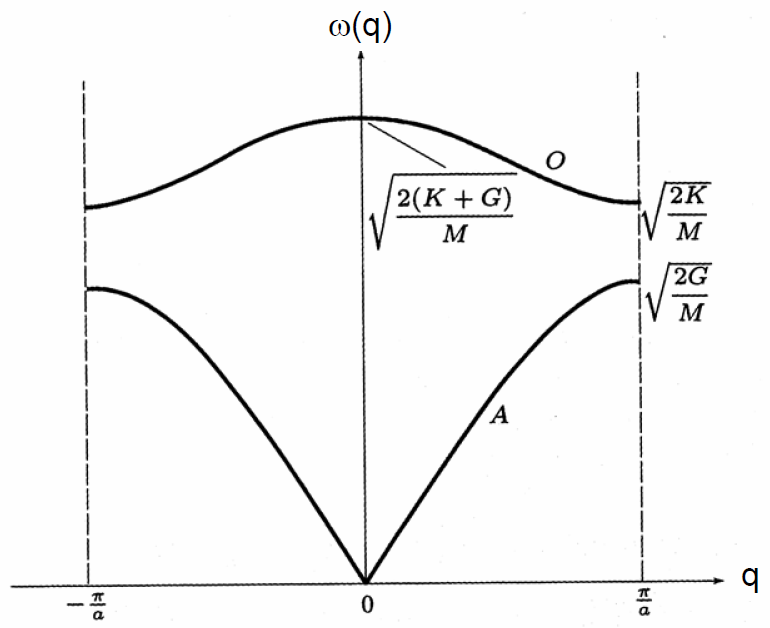
\includegraphics[width=8cm]{blatt04-9c.png}
\caption{Dispersionsverlauf, dem Skript der Vorlesung entnommen}
\end{wrapfigure}

\end{document}

